%
% 計測自動制御学会システム・インテグレーション部門学術講演会2012原稿サンプルファイル
%                                           October 4, 2012
% Based on 計測自動制御学会システム・情報部門学術講演会2012原稿サンプルファイル
%                                           April 28, 2012
% Based on 第7回計測自動制御学会制御部門大会原稿サンプルファイル
%                                           October 18, 2007
% Based on 第5回計測自動制御学会制御部門大会原稿サンプルファイル
%            近野敦 konno@space.mech.tohoku.ac.jp    March 05, 2005
%

\documentclass[10pt,a4paper]{jarticle}
\usepackage{tc2015_utf}
\usepackage[dvipdfmx]{graphicx,color}
\usepackage[fleqn]{amsmath}
\usepackage{algorithm,algorithmic}
\usepackage{amssymb,epsfig}
\usepackage{ascmac}

\usepackage{bm}
\usepackage{ascmac}
\usepackage{pifont}
%\usepackage{multirow}
\usepackage{enumerate}
%\usepackage{cases}
\usepackage{type1cm}
\usepackage{here}

\def\vec#1{\mbox{\boldmath$#1$}}
\def\vector#1{\mbox{\boldmath $#1$}}

\newcommand{\argmax}{\mathop{\rm arg~max}\limits}
\newcommand{\argmin}{\mathop{\rm arg~min}\limits}
\newcommand{\umax}{\mathop{\rm max}\limits}

\def\R{{\Bbb R}}
\def\Z{{\Bbb Z}}

\renewcommand{\topfraction}{0.8}
\renewcommand{\bottomfraction}{0.8}
\renewcommand{\dbltopfraction}{0.8}
\renewcommand{\textfraction}{0.1}
\renewcommand{\floatpagefraction}{0.8}
\renewcommand{\dblfloatpagefraction}{0.8}
\setcounter{topnumber}{3}
\setcounter{bottomnumber}{3}
\setcounter{totalnumber}{3}

\begin{document}
\title{\fontsize{16pt}{0pt}\selectfont 九州工業大学におけるつくばチャレンジへの取り組み}
\author{\fontsize{12pt}{0pt} 有田 裕太(九州工業大学)~ 田中 良道(九州工業大学) \\ ~ 森田 賢(九州工業大学)~西田 健(九州工業大学)}
\engtitle{
   \fontsize{16pt}{40pt}\selectfont 
}
\engauthor{
  \fontsize{12pt}{0pt}\selectfont Arita Yuta(Kyutech), Tanaka Ryodo(Kyutech), \\ Morita Masaru(Kyutech) and Nishida Takeshi(Kyutech)
}

\abstract{
\fontsize{9pt}{0pt}\selectfont
}

\maketitle\thispagestyle{empty}
\pagestyle{empty}

\section{はじめに}
\label{sec:intro}
我々は,九州工業大学工学部の学部生を中心としたロボット開発チームであり,屋内外の移動を行う福祉ロボットの開発に取り組んでいる.このような福祉ロボットに必要とされる機能には,案内・荷物の運搬・搭乗者の安全な搬送・周囲環境に対する回避,発見,追従動作などが挙げられる.そこで我々は市販の電動カートを改造し,これらの作業を行うための福祉ロボット(KIT-C3)を開発した.しかし,このロボットでは屋内を走行する際には大きすぎるため,比較的小さく,小回りもきくロボット(KIT-C4)の開発も行った.本稿では,これらのロボットの開発とつくばチャレンジ2015での実験結果について報告する.

\section{ロボットの構成}
\subsection{ハードウェア構成}
\subsubsection{KIT-C3}
本ロボットでは,シニアカータウンカート(スズキ株式会社製TC1A4)の走行系を用いた.シニアカーの走行系は,バッテリーや走行安定性や防水性など,様々な面で屋外での走行機能や信頼性が高く,ほとんど故障などの問題が発生することが無い.さらに,ホイールレングスが1[m]程度あるため,直進走行性能が高く,自動走行制御に対して再現性が高いというアドバンテージがある.一方で,つくばチャレンジの他のチームの小型走行ロボットよりは比較的車体が大きく,車重も97[kg]と重い.Fig.\ref{213021_18Dec14}にKIT-C3の外観を示す.

\begin{figure}
  \centering
  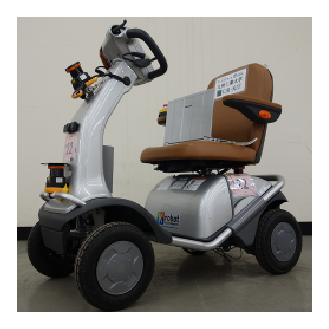
\includegraphics[width=7cm]{fig/eps/kitc3.eps}
  \caption{KIT-C3の外観}
  \label{213021_18Dec14}
\end{figure}

\subsection{センサ構成}

\subsubsection{KIT-C3}
KIT-C3は環境観測用センサとして前方にLRF(北陽電気製UTM-30LX)を2台,後方にもLRF(北陽電気製URG-04LX-UG01)を1台搭載している.また,ロボットの状態観測用センサとしてロータリーエンコーダ(MUTOH製UM-125)をステアリング軸に1つ取り付けている.このセニアカーの後輪は独立に2つのモータとエンコーダが搭載されており,そのエンコーダ情報をマイコンにより取得している.

\subsection{全体の構成}
\subsubsection{KIT-C3}
ロボットへの速度指令やロータリーエンコーダの処理用マイコンとして iXs Research 社のiMCs01を用いた.シニアカーの速度制御はiMCs01で0-5[V]の電圧を生成しシニアカーのアクセル信号部に印加することで実現している.またステアリング操舵のためのステッピングモータの制御にArduino Unoを用いた.制御用PCはラップトップPCを用いており,OSはUbuntu 14.04を使用した.以上の構成の概要をFig.\ref{225251_18Dec14}に示す.ラップトップPCとiMCs01やURGとはUSB接続である.また,Fig.\ref{213021_18Dec14}における破線はシニアカーの制御基板によって制御されていることを表す.

\begin{figure}
  \centering
  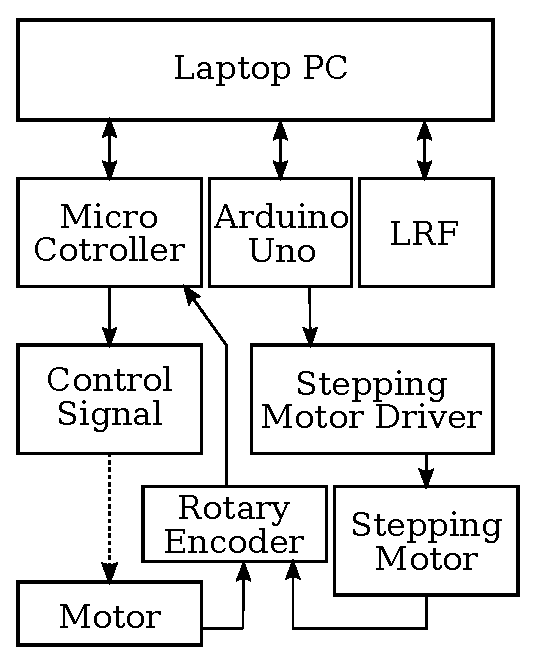
\includegraphics[width=6cm]{fig/eps/kitc3_overview.eps}
  \caption{KIT-C3のシステムの概要}
  \label{225251_18Dec14}
\end{figure}

\section{ソフトウェアの構成}
\subsection{ROS}
今回,2台のロボットを開発するにあたり,できる限りソフトウェアの再利用性と共通化を図るためにROS(Robot Operating System)を導入した.また,ROSのnavigationスタックを利用し,自律走行を行った.なお,ROSのバージョンはIndigoを用いた.

\subsection{走行手法}
予め環境地図を作成し,環境地図上にWaypointsを数メートル毎に設定し,それらを順に辿っていくようにして自律移動を行った.Waypointsの設定はROSの可視化ソフトウェアrviz上でクリックやドラッグ操作で設定できるパッケージを開発しこれを用いた.経路生成および障害物回避にはmove\_baseパッケージを用いた.また,自己位置推定にはAMCL(AdaptiveMontecalro Localization)を用いた.昨年は前方下に取り付けた1台のLRFで自己位置推定を行っていたが,今年は前方と後方に取り付けた2台のLRFで自己位置推定を行った.

\subsection{環境地図}
環境地図はROSのパッケージ化されたgmappingを用いて作成した.環境地図は10[cm]四方の占有格子地図とした.環境地図作成に用いたセンサは昨年はLRF1台とホイールオドメトリのみであったが,今年は自己位置推定同様に前方と後方に取り付けた2台のLRFとホイールオドメトリを利用して作成した.これにより大清水公園などでも比較的精度の高い地図を短時間で作成することができた.また,確認走行を完了したあとは大清水公園と公園の外でそれぞれ地図を作成し画像編集ソフトを用いて1つに統合したものを用いた.作成した地図をFig.\ref{204704_18Dec14}に示す.作成された地図は閉じていないものの,重なりは生じていないため,自己位置推定などには問題なく使用できた.作成された地図が歪んでいる原因としてオドメトリがずれていることが挙げられる.オドメトリパラメータの修正や,ジャイロセンサを組み合わせることでオドメトリを高精度化できれば更に高精度な地図を作成できると考えられる.

\begin{figure*}
  \centering
  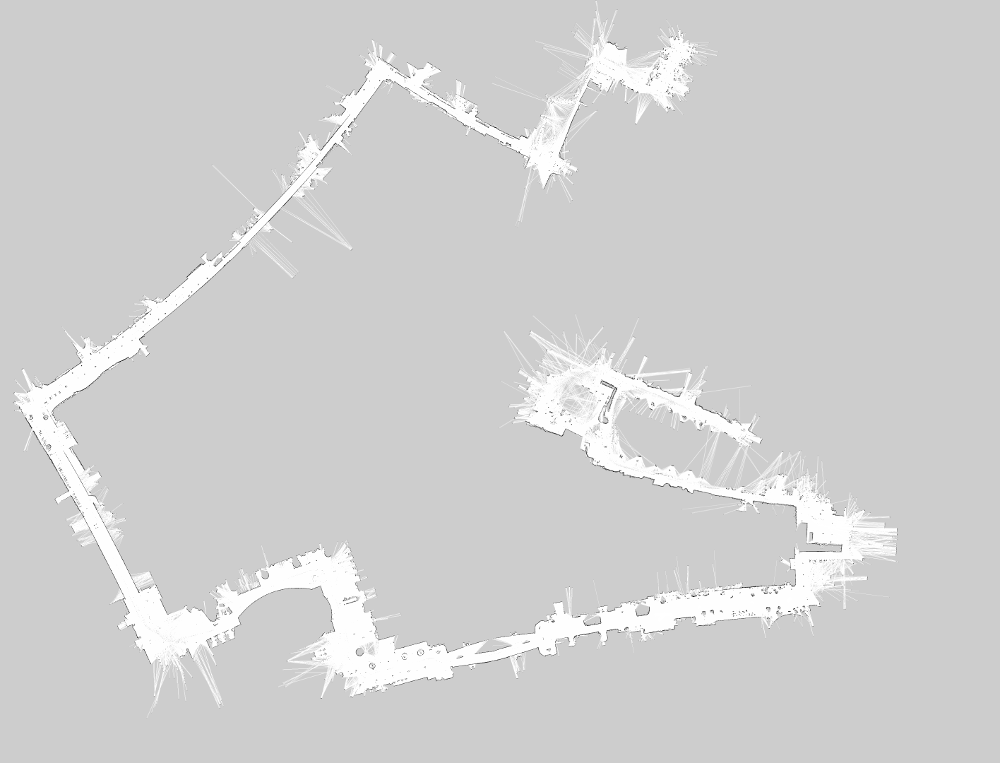
\includegraphics[width=14cm]{fig/png/gridmap.png}
  \caption{KIT-C3の作成した環境地図(コース全域)}
  \label{204704_18Dec14}
\end{figure*}
\subsection{下方段差検出}
環境地図作成時点では存在しない障害物の回避にはROSの local\_planner パッケージを利用したが,下方段差検出における問題が発覚した.
KIT-C3には,下り階段や急激な下り坂への進入を回避するために,地面方向に照射するLRF(下方照射LRF)が搭載されている.ところが,そのような段差で得られる下方照射LRFの生データを local\_planner に入力しても,
段差を回避する経路を獲得できない.この理由は,次に示すlocal\_plannerの仕様とLRFの特性の不一致にあり,具体的には,
1)  local\_planner は地面よりも高い場所に位置する物体を障害物と検知する,すなわち下方照射LRFの出力距離が地面までの距離より小さいことを検知するが,2) 実際には段差において下方照射LRFは地面までの距離よりも大きい距離を出力する,というものである.
つくばチャレンジ2014では正にこの問題のため,段差に進入の直前でロボットを停止させた経緯があった.

そこで今年度は,下方照射LRFが地面までの距離よりも大きい値を出力した場合,それをlocal\_plannerが障害物と認識できる値に人為的な変更を加える機能を追加した.この様子をFig.\ref{lower_step_detector} に示す.

最後に,本機能の工夫点について述べる.下方段差を機能させるためには,ロボット,LRF,地面との位置関係や,環境に合わせたLRFの感度の調整が必要となることが予想されたため,細かくパラメータを調整できる仕様を定めて実装を行った.
これにより,事前の検証において,屋内では段差検出ができたが屋外で検出ができないという問題が発生したが,パラーメータ調整だけでこの問題を容易に解決することができた.

\begin{figure}
    \centering
    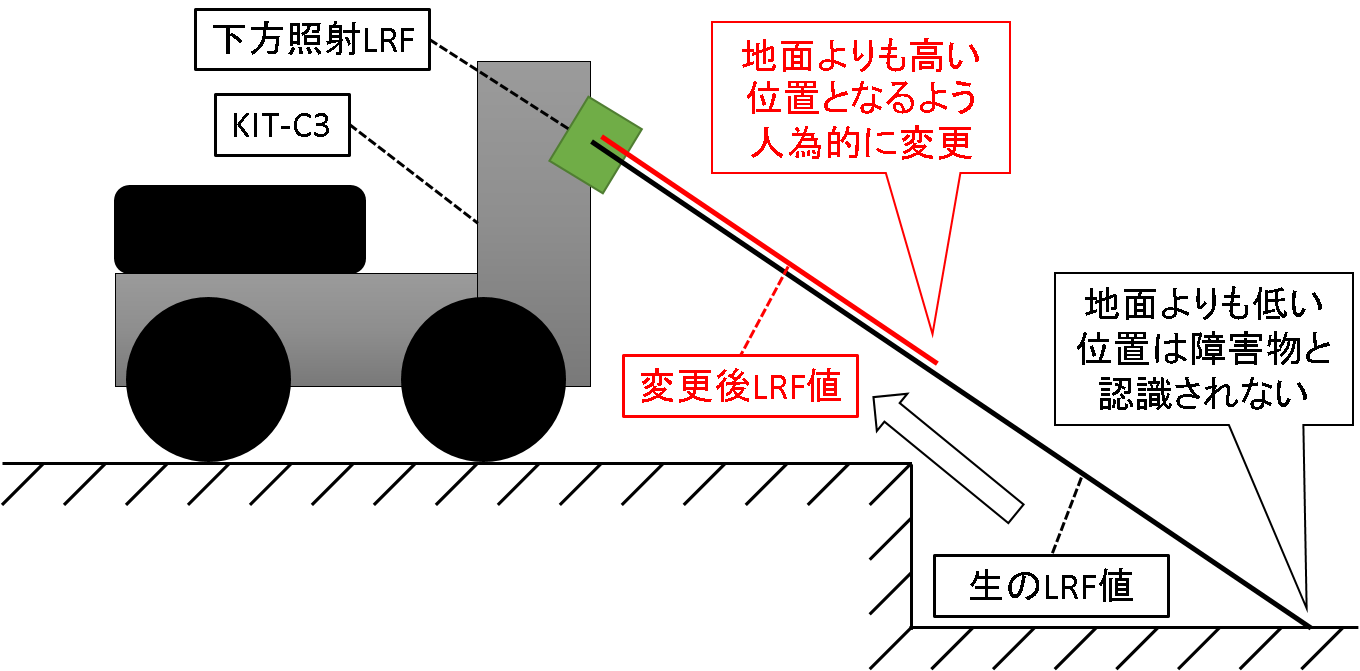
\includegraphics[width=8cm]{fig/png/lower_step_detector.png}
    \caption{KIT-C3の下方段差検出}
    \label{lower_step_detector}
\end{figure}

\subsection{遠隔監視システム}
つくばチャレンジの注意事項等について,「ロボットの位置や状況のステーションにおけるモニタリング」を強く推奨すると明記されている.我々は本要求事項を達成する遠隔監視システムを構築したので,その機能とネットワーク環境について述べる.
ただし,本システムは大会当日に機能させることが出来なかったため,以下では開発時の情報を用いて説明する.

初めに,遠隔監視について述べる.監視画面として,ロボットの現在姿勢を地図上に表示させる形式を採用した.現在姿勢,あるいは現在姿勢と経路履歴の両方,を選択的に表示できるようにした.現在姿勢を表示した様子をFig.\ref{monitor}に示す.なお,同図で画像の一部のみを拡大をしている箇所は説明のために加工を施したもので,実際のシステムでは背景の大域地図上にロボットの姿勢が表示されるのみである.
\begin{figure}
    \centering
    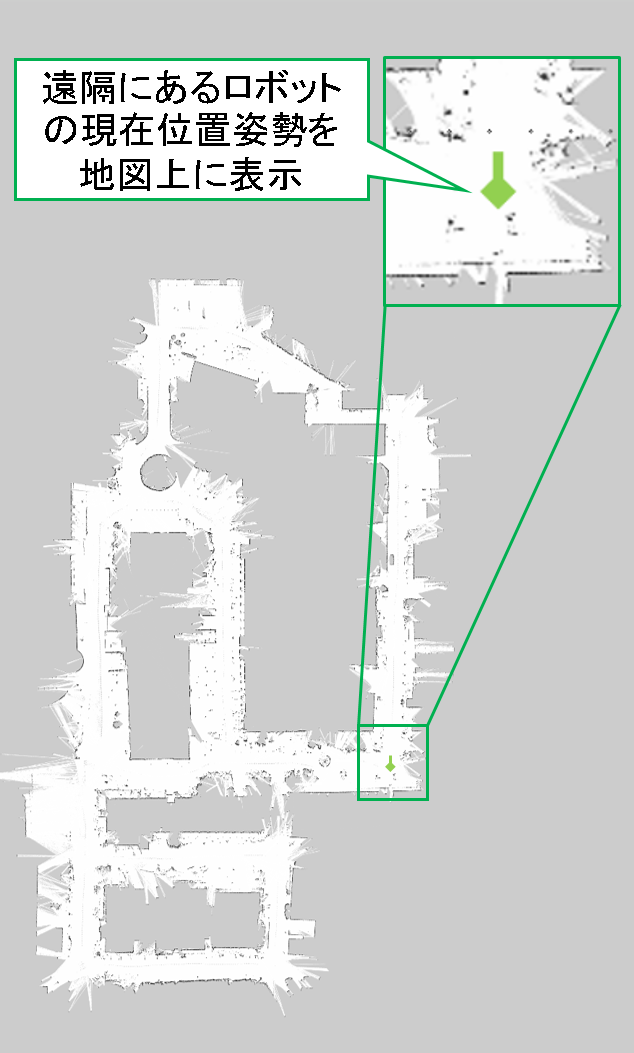
\includegraphics[width=6cm]{fig/png/monitor.png}
    \caption{遠隔監視システムで地図上に現在姿勢を表示させた様子.}
    \label{monitor}
\end{figure}

次に,通信環境について述べる.監視端末とロボット間の通信回線として商用モバイル回線を利用し,VPNで接続を行った.VPNシステムとして,OpenVPNを採用した.遠隔監視PCをサーバ,ロボットをクライアントとしてVPNネットワークを構成し,ROS ネットワークとの連携させることで,遠隔監視を実現した.

ここで,工夫点について記述する.本システム開発当初,本構成でROSの可視化ツールであるrvizによる監視を試みたところ,rvizはリアルタイムに更新される位置情報を全て取得しようと試みるのだが,商用回線の通信速度ではその情報量に対応しきれず,情報の更新漏れが頻繁に発生してしまった.また,パケット通信容量が膨大で,契約した通信回線の上限を容易に超えてしまう恐れがあり,遠隔監視そのものが実現できなくなる懸念があった.
そこで,ロボットが一定距離を移動する毎に,自身の位置を監視端末に送信する仕様に変更することで,更新漏れとパケット通信料の問題を解決した.検証段階では送信間隔5[m]毎に設定したが,ロボットの位置を追跡するには十分な周期であった.

最後に,本機能の展望を記述する.ネットワークシステムを独自で構築したため,位置に限らず任意の情報を遠隔監視するための基盤技術を確立できた.期待される機能の例として,ロボットの現在速度,電池残量,検出した人物の画像等といった,遠隔監視に有益な情報表示機能が挙げられる.

\section{結果と考察}
\subsection{実験走行}
\subsubsection{KIT-C3}
LRFを2台用いることによって環境地図が安定して作成できるようになったため,一度手動で操作してデータ取りを行った後,すぐに地図作成を完了することができた.また,実験走行では横断歩道手前まで何度か走行できたものの,横断歩道を通過する実験を行うことが出来なかった.横断歩道へ侵入する際の段差が想定よりも大きく,車体が前のめりに傾いた際に地面を障害物として認識してしまっていた.他にも,コース後半の橋を渡ったあとの下り坂でも同様の現象が発生したことがあった.

\subsection{本走行結果}
\subsubsection{KIT-C3}
本走行では雨だったものの,ラップトップPCをビニール袋で覆う以外には特に防水処理は行っていない.LRFが雨を障害物として認識することがあり,頻繁に一時停止するものの,順調に走行し,横断歩道手前までの約1420[m]自律走行を行った.しかし,横断歩道手前で一時停止出来なかったため,オペレータが緊急停止スイッチを押し,停止させた.
横断歩道手前のwaypointに到達したら一時停止するような処理を実装していたが,waypointの位置の設定ミスが原因だった.横断歩道手前での実験が不十分だったことが設定ミスの原因である.

昨年からハードウェア構成やソフトウェア構成をほとんど変更していないものの,地図作成や自己位置推定に用いたLRFを1台から2台に変更し,360度から情報を得ることができるようになったことで格段に安定性を大きくすることが出来た.また,オドメトリの精度向上も自己位置推定の安定性向上につながった.しかしながら,広い場所では自己位置推定が安定しない場合があったため,3DLidarなどを利用した自己位置推定を利用して解決を図りたい.

また,今回は完走を目標としたため人物発見には取組めていない.次回の参加では人物発見を行い,課題の完全達成を目指したい.


\section{開発状況などに関して}
我々のチームは実験走行になかなか参加出来ないため,学内での実験を積み重ねてきた.学内の実験においても約1000[m]程度の自律走行が安定してできていた.しかし,学内での実験では他のロボットや未知の障害物などは少なく,道幅は広く,起伏が殆ど無い環境だったためつくばチャレンジの環境では上手く行かないことがあった.本番前の実験走行ではこの辺りの調整が大変だった.


\section*{謝辞}
つくばチャレンジ実行委員会やつくば市の方々にはつくばチャレンジのような貴重な実験の機会を与えていただき感謝いたします.



% \begin{thebibliography}{9}% 文献が10以上のとき99,10未満のとき9
 
% \end{thebibliography}

%\appendix
%\section{}


\end{document}
